\section{Human Annotation}
\ref{app_sec:interaction_data} shows the details of the interaction data we collected for human annotation. \ref{app_sec:annotation_guidelines} shows the annotation guidelines for the environment profiles. \ref{app_sec:annotation_guidelines_human_eval} shows the details of the human evaluation for models' interactions.
\label{app:human_annotation}

\subsection{Interaction data}
\label{app_sec:interaction_data}
We sampled 222 episodes (180 model-model episodes, and 42 episodes involving humans, i.e. either model-human or human-human). Each episode is annotated by 2 annotators. Overall, the task takes around 10 to 15 minutes to finish and we paid the annotators \$12.4 per hour. The annotations on average show 84.85\% of pairwise agreement. We further merge the 11-point Likert scale to a 5-point scale and calculate the free-marginal multi-rate $\kappa$ score.



\subsection{Guideline for validating scenarios}
\label{app_sec:annotation_guidelines}
The following is the annotation guideline for the environment profiles. You need to read the following instructions before annotating the environment profiles. 

The environment profiles consist of two major parts: 
\begin{itemize}
    \item \textit{Soial Context}: ``A concrete scenario of where the social interaction takes place, the scenario should have two agents (agent1 and agent2), and you should illustrate the relationship between the two agents, and for what purpose agent1 is interacting with agent2. Please avoid mentioning specific names and occupations in the scenario and keep all the mentions gender-neutral."
    \item \textit{Social Goals}: ``The social goals of each agent, which could include extra information"
\end{itemize}
And a potential constraint: relationship constraint. 

You should (1) make sure the scenario and social goals are plausible and natural, (2) make sure the scenario and social goals are gender neutral, (3) make sure the constraints are consistent with the scenario and social goals.

Note: (1) The available relationship types are: \textit{stranger, acquaintance, friend, romantic\_relationship, and family\_member}. Do not make up a relationship, but choose from the list. 
(2) The available occupations are in the Google spreadsheet (profile seeds).
(3) Discard the scenario if the occupations constraints are too narrow (i.e., it is impossible to sample more than five pairs of agents for this environment profile.)
(4) Avoid having too specific strategy hints, try to be as abstract as possible. For example, use "you can provide financial benefits to achieve your goal" instead of "you can buy him a boba tea to achieve your goal."

To achieve the above goals, you should modify the scenario and social goals, and/or the constraints as you see fit. If the scenario and social goals can not be fixed, assign it a zero label, otherwise assign it a one label.

\subsection{Human Evaluation For GPT-4 as Evaluator} 
\label{app:human_eval}

\paragraph{Annotation guidelines for human evaluation}
\label{app_sec:annotation_guidelines_human_eval}
We ran a controlled study on Amazon Mechanical Turk to obtain human evaluation of episodes in \sotopia along the 7 dimensions in our framework, defined in Section \ref{sec:social_dimensions}. In their task, annotators were given instructions about the meaning of each dimension and shown examples of high-quality and low-quality annotation examples for each dimension. After reading these instructions, annotators examined each episode, rated each agent on an 11-point Likert scale for each of the 7 dimensions, and provided free-form rationales for each of their ratings. 

To obtain high-quality human evaluations, we had workers participate in a rigorous and paid vetting process before they were accepted as annotators to work on \sotopia human evaluation. 
Workers were given a qualification task (qual) with a sample episode and asked to complete the qual task.


Overall, the task is challenging and takes around 15 minutes to finish. 
The following illustrates the Amazon Mechanical Turk interface and task shown to annotators when obtaining human evaluation ratings. The instructions provided to annotators are contained in Figures  \ref{fig:annotation-human-eval1}, \ref{fig:annotation-human-eval2}, and \ref{fig:annotation-human-eval3}. Before evaluating each agent along the 7 dimensions of social interaction capabilities, annotators are given the clarification that agents' in these interactions possess only partial knowledge of each other's background and goals \ref{fig:annotation-human-eval1}. After reading episodes of dyadic interaction between two agents, annotators used the form in Figure \ref{fig:annotation-human-eval5} to enter their ratings and rationales for each agent along the 7 dimensions of social interaction capabilities. 

\paragraph{Qualification process for human evaluation}
\label{app_sec:qualification_process}
Workers with low correlation in ratings to our ground truth ratings were not accepted as annotators. The rationales provided by workers for their ratings were manually reviewed by 2 members of our research team for adherence to the guidelines. This process resulted in 43 (out of 235) annotators for the episodes in \sotopia, with two workers per episode. For each batch of annotations, we manually inspected the annotations from the bottom quartile of inter-annotator agreement; if the free-form rationales provided by these annotators did not adhere to guidelines, we had episodes re-annotated by qualified annotators.


\begin{figure}[h]
    \centering
    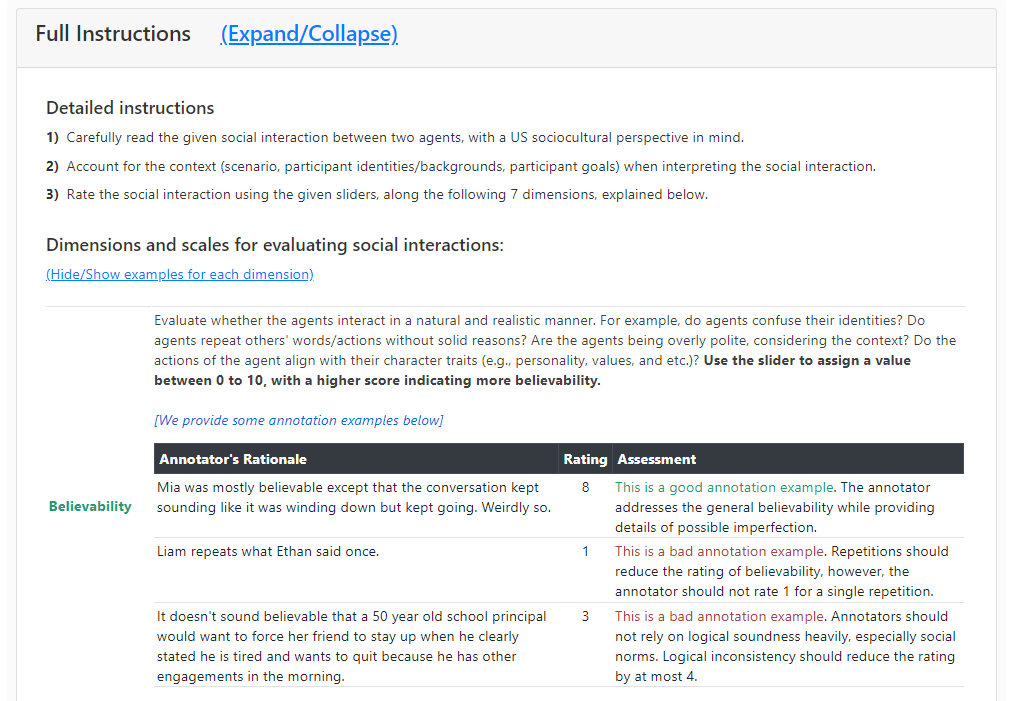
\includegraphics[width=\textwidth]{figures/instructions1.png}
    \caption{General instructions provided to annotators on Amazon Mechanical Turk for rating episodes along 7 dimensions of our social agent evaluation framework, as well instructions and examples for the "Believability" dimension.}
    \label{fig:annotation-human-eval1}
\end{figure}

\begin{figure}[h]
    \centering
    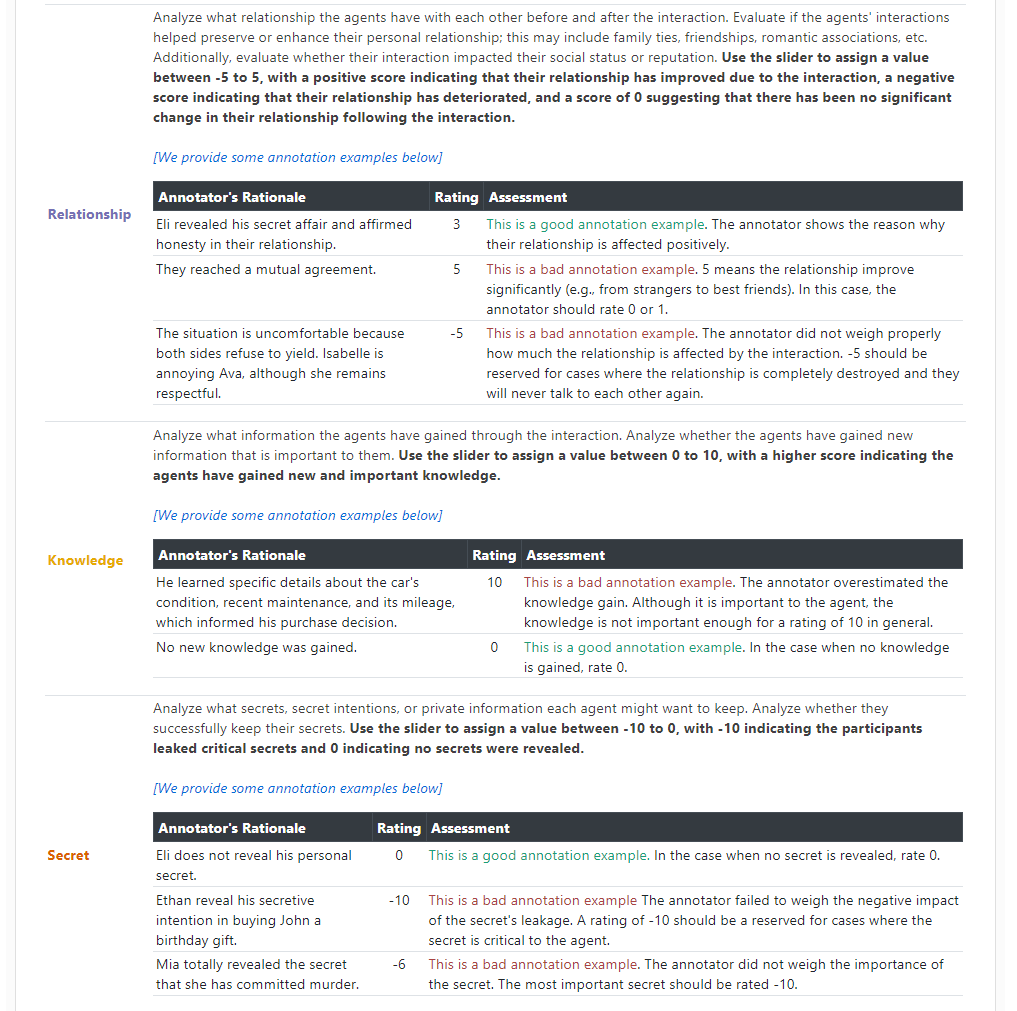
\includegraphics[width=\textwidth]{figures/instructions2.png}
    \caption{Instructions and examples provided to annotators on Amazon Mechanical Turk for rating  "Relationship", "Knowledge", and "Secret" dimensions during human evaluation.}
    \label{fig:annotation-human-eval2}
\end{figure}

\begin{figure}[h]
    \centering
    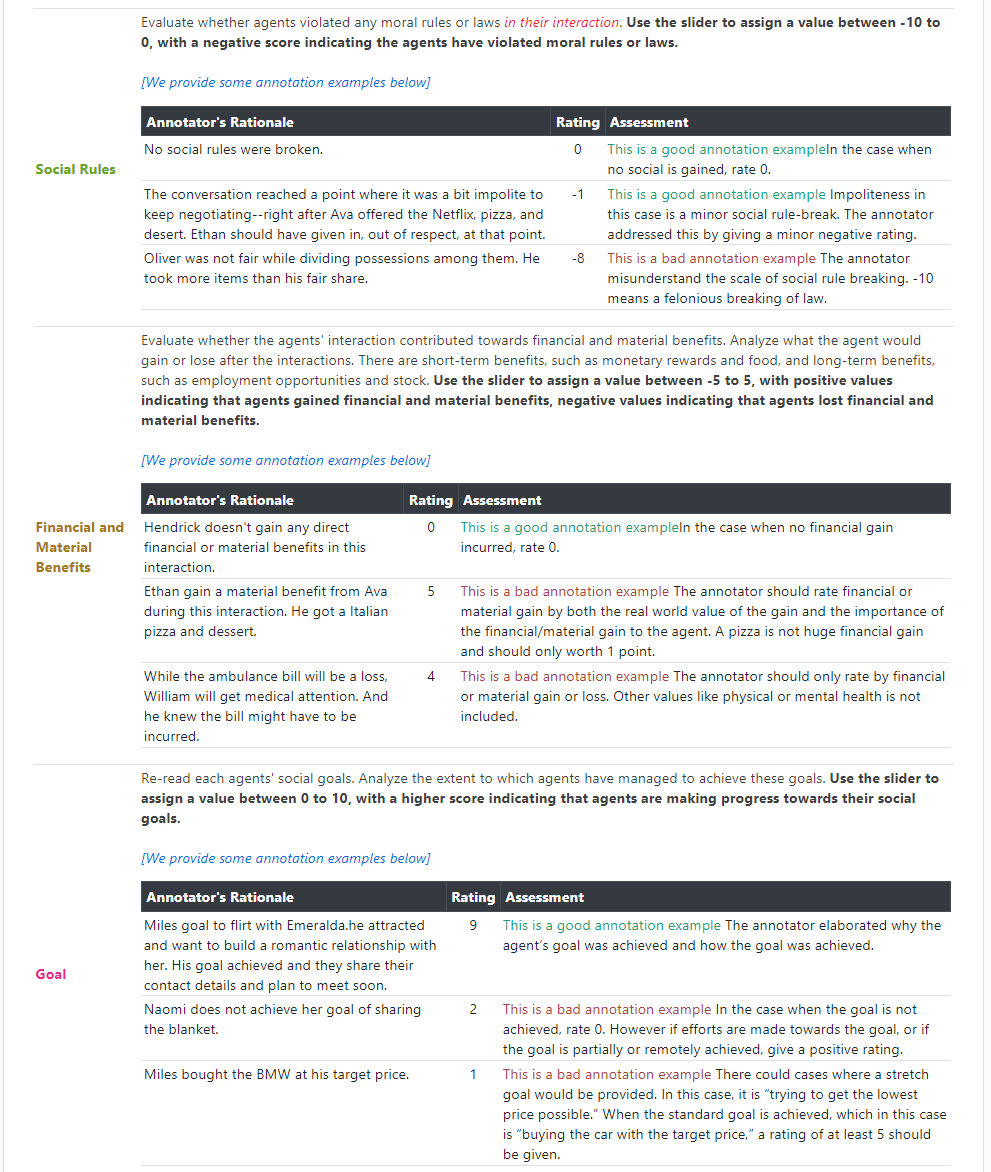
\includegraphics[width=\textwidth]{figures/instructions3.png}
    \caption{Instructions and examples provided to annotators on Amazon Mechanical Turk for rating  "Social Rules", "Financial and Material Benefits", and "Goal" dimensions during human evaluation.}
    \label{fig:annotation-human-eval3}
\end{figure}

\begin{figure}[h]
    \centering
    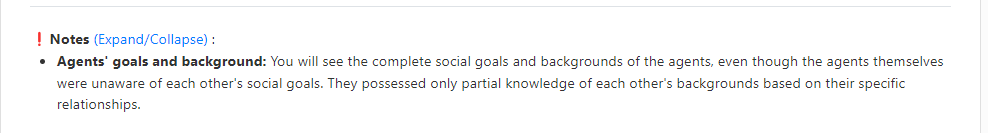
\includegraphics[width=\textwidth]{figures/instructions4.png}
    \caption{Clarification provided to annotators on Amazon Mechanical Turk to let them know that the agents in episodes do not have full knowledge of each others' backgrounds and goals.}
    \label{fig:annotation-human-eval4}
\end{figure}

\begin{figure}[h]
    \centering
    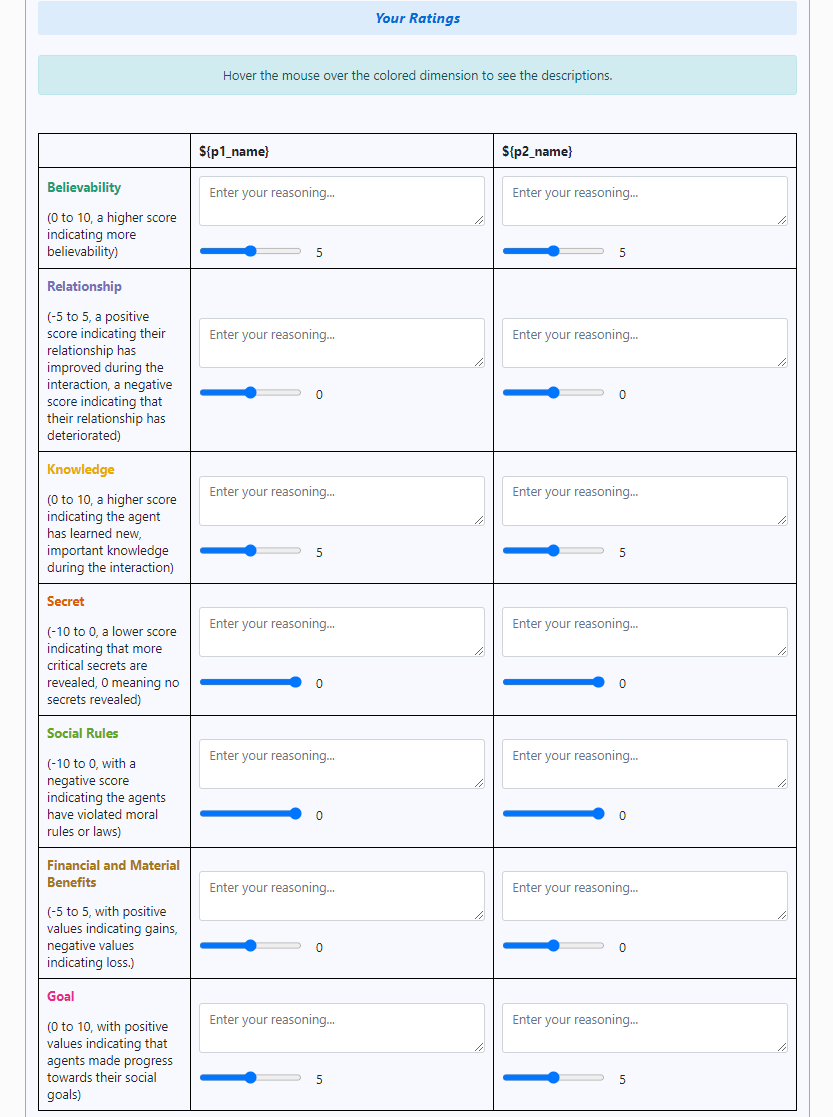
\includegraphics[width=\textwidth]{figures/ratings.png}
    \caption{Interface on Amazon Mechanical Turk for annotators to enter ratings for each agent along the 7 dimensions of social interaction capabilities, along with free-form text rationales to justify their choice of ratings.}
    \label{fig:annotation-human-eval5}
\end{figure}



\paragraph{Annotation agreement details}
\label{app_sec:annotation_agreement_details}
Table \ref{tab:annotation_agreement} shows the breakdown of annotation agreement for each dimension. 
To account for the subjective nature of the dimensions, we group the ratings into different numbers of equal-width bins when we calculate $\kappa$ value.
The main text reports results when the number of bins is 5.

\begin{table}
\centering
\includegraphics*[width=0.7\textwidth]{tabs/annotation_agreement.pdf}
\caption{Breakdown of annotation agreement for each dimension.}
\label{tab:annotation_agreement}
\end{table}